The Advanced Laser Interferometer Gravitational-Wave Observatory (aLIGO) is part of an international effort to detect gravitational waves. 
The search will resume later this year with the two aLIGO sites in Washington and Louisiana, which will ramp up to full design sensitivity over the following few years.

\section{Basic layout of aLIGO}

In its simplest form, aLIGO is a Michelson interferometer with Fabry-P\'erot cavities for arms (see figure \ref{fig:michelson}). In each Fabry-P\'erot cavity, the mirror closer to the Michelson beam splitter is called the input test mass (ITM) and the other mirror is called end test mass (ETM).

When a gravitational wave passes through the detector, it causes changes in the distance between the ETM and ITM in each cavity. Because the wave is quadrapolar, the changes in the x direction will have the opposite sign of the changes in the y direction. This causes a relative phase shift in each of the arms in opposite directions. When they recombine at the beam splitter, the phase shifts cause changes in the interference between the two beams, changing the amount of power at the the output port. We can detect these power fluctuations to reconstruct the phase shift and thus the strain, $h=\Delta L/L$ experienced by the interferometer due to the gravitational wave. We then use techniques like matched filtering to compare the strain signal from the interferometer to models of expected signals to search for events hidden in the noise background of the interferometer. 


\begin{figure}[htp]%
\center
\includegraphics[width=.5\textwidth]{figures/introduction/Michelson}%
\caption[Simplified LIGO Layout]{In its simplest form, aLIGO is a Michelson interferometer with Fabry-P\'erot cavities for arms. Light from the laser is split by the beam splitter (BS), then enters the arm cavities through the input test masses (ITMX and ITMY). Power builds up in the cavity between input and end test masses (ETMX and ETMY). When a gravitational wave passes through the detector, it shifts the phases of light in the two arms in opposite directions. Because the cavity is over-coupled ($r_{ITM}<r_{ETM}$), light leaves the arm cavities and goes back to the BS. The phase-shifted light from the two cavities interferes at the BS, producing the error signal that we measure with a photodiode.}%
\label{fig:michelson}
\end{figure}

